\subsection{FeSe diatomic molecule (NE-AIDMD)}

Transition metal systems are an especially difficult case for most electronic structure methods, and therefore, are an 
important test case for AIDMD. 
Diffusion Monte Carlo (DMC) is particularly useful in transition-metal systems, where is has been shown to improve the description of energy gaps for the types of orbital excitations used to sample the Hilbert space~\cite{lucas}.
Given the expense of large DMC calculations, finding models consistent with DMC would be valuable for studying extended transition metal systems.
Additionally, transition metal systems involve competing interactions that can give rise to novel phenomena. 
Utilizing matching pursuit and AIDMD to find minimal descriptions can offer a way to quantify the relative importance of different interactions.

As a test of AIDMD for transition metal systems, we consider an FeSe diatomic molecule with atomic separation 2.43 \AA~in the $z$-direction.
To our knowledge, this FeSe diatom does not exist in nature, but nevertheless serves as a simple illustration of a model for the interaction between a transition metal and a ligand.
The bond distance is chosen to match the unconventional superconductor, FeSe~\cite{fese}, and therefore offer insight into a model description for that system in future calculations.

We consider a multiband Hubbard model including one iron $s$, five iron $d$ states, and three selenium $p$ states:
\begin{align*}
  H 
  &=
  \epsilon_{d_{xy}} \sum_{\eta} (n^{d_{xy}}_{\eta}  + n^{d_{x^2-y^2}}_{\eta})
  +
  \epsilon_{d_{z^2}} \sum_{\eta} n^{d_{z^2}}_{\eta} 
  +
  \epsilon_s \sum_{\eta} n^{s}_{\eta} 
  +
  \epsilon_{p_{z}} \sum_{i,\eta} n^{p_{z}}_{i,\eta} 
  \\
  &+ 
  t_{\sigma,d} \sum_{\eta} \left( d_{z^2,\eta}^{\dagger} p_{z,\eta} + \text{h.c.} \right)
  +
  t_{\sigma,s} \sum_{\eta} \left(s_{\eta}^{\dagger}  p_{z,\eta} + \text{h.c.} \right)
  \\
  &+ 
  t_{\pi} \sum_{\eta} \left( d_{xy,\eta}^{\dagger} p_{x,\eta} + d_{yz,\eta}^{\dagger}  p_{y,\eta} + \text{h.c.} \right)
  \\
  &+
  U_d \sum_{i} n^{d}_{i,\uparrow} n^{d}_{i,\downarrow} 
  +
  J_d \sum_{i\ne j} S_i \cdot S_j.
  +
  E_0
\end{align*}
Here, $\eta$ represents the spin index and $i$ represents orbital index.
The $\epsilon_i$ terms represent single-particle orbital energies, while the $U_d$ is an on-site interaction among the $d$ orbitals and the $J_d$ is a Hund's coupling among the $d$ orbitals.
$E_0$ is an overall energy shift compared to the \textit{ab initio} hamiltonian.
This set of parameters was chosen based on the matching pursuit method described in Sec.~\ref{sec:theory}.
We stop selecting terms in the model when all other descriptors do not correlate with the residuals of the fit.
For example, $U_p$, an on-site interaction for the Se $p$-electrons, does not correlate with the residuals, and therefore was excluded from the model.
The states sampled consisted of singles and doubles excitations from PBE0 calculations with total spin 0, 2, and 4, which were then relaxed via a DMC projection.

The parameters resulting from NE-AIDMD are presented in Table~\ref{tab:fese}, shown in the order selected by matching pursuit. 
The error of the model including only parameters in or above the row is shown in the column labeled ``RMSE.''
The sign of $J$ is consistent with Hund's rules. 
The signs of $t_{\sigma,d}$ and $t_{\sigma,s}$ are positive, because Se is located in positive $z$ with respect to Fe. 
Likewise $t_\pi$ is negative corresponding to positive overlap integrals, and is smaller than $t_\sigma$ in magnitude.
The $\epsilon_i$ states represent energies of the single particle orbitals relative to the energy of $d_{xz}$, $d_{yz}$, $p_x$, and $p_y$, which are likely close in energy.

The matching pursuit algorithm would suggest that minimal models can be built by disregarding the descriptors added in later steps.
In this approach, $J$ is considered the most important parameter in the model, and an absolute minimal model for the system would be $H_\text{minimal} = E_0 + J_d \sum_i S_i \cdot S_j$. 
Such a model would have a RMSE 1.11 eV. 
According to matching pursuit the next most important interactions to include are (1) hopping between $d_{z^2}$ and $p_z$, (2) on-site $d$ Coulomb interactions, and (3) hopping between the $4s$ and the $p_z$, and so on. Including these degrees of freedom brings the RMSE to 0.75 eV.
Further improvements are possible with additional interaction terms; however, the drops in RMSE diminish. 
In this way MP would suggest that the most important interactions in the system are Hund's coupling, hopping with Se, and on-site Coulomb repulsion, in that order.
This observation is consistent with the several studies in the literature, which find Hund's coupling in bulk FeSe to be an important part of its description~\cite{hunds}.
A comparison of the model and \textit{ab initio} energies is shown in Fig. \ref{fig:fese}.

\begin{table}[ht]
\label{tab:fese}
\centering
\begin{tabular}{|c|c|r|c|}
  \hline
  MP step & Selected parameter & Final Value [eV]  & RMSE [eV] \\
  \hline
  1 & $E_0$                    &  -3620.9(4) & 1.53 \\
  2 & $J$                      &  -0.45(4)   & 1.11 \\
  3 & $t_{\sigma,d}$           &  3.0(2)     & 1.02 \\
  4 & $U_d$                    &  2.6(1)     & 0.89 \\
  5 & $t_{\sigma,s}$           &  2.1(2)     & 0.75 \\
  6 & $\epsilon_{d_{xy}}$      &  -0.36(7)   & 0.69 \\
  7 & $\epsilon_{s}$           &  2.1(2)     & 0.66 \\
  8 & $\epsilon_{p_z}$         &  -1.4(2)    & 0.61 \\
  9 & $t_\pi$                  &  -0.7(1)    & 0.57 \\
  10& $\epsilon_{d_{z^2}}$     &  -0.4(1)    & 0.56 \\
\hline
\end{tabular}
\caption{
  \BDB{Problem: this is a bit misleading because the parameter values change slightly during the MP steps, needs discussion}
    Downfolding parameters for FeSe diatomic molecule. 
    The parameters are shown in the order chosen by matching pursuit (MP), so that $J$ correlated most strongly with the energy, $t_{\sigma,d}$ correlated most strongly with the error in the $E_0$-$J$-model, $U_d$ correlated most strongly with the error in the $E_0$-$J$-$t_{\sigma,d}$ model, and so on.
    The final value of the parameter on the 10-th MP step is shown in "Final Value."
    Note that the parameters change slightly as the MP progresses, but important parameters such as $J$ and $U_d$ by only around a few percent.
    The RMSE for the model including parameters chosen by MP up to that step are shown in the final column. 
    Parameters chosen by MP first tend to reduce the error more significantly than those chosen later. 
  }
\end{table} 

\begin{figure*}[htb]
\centering
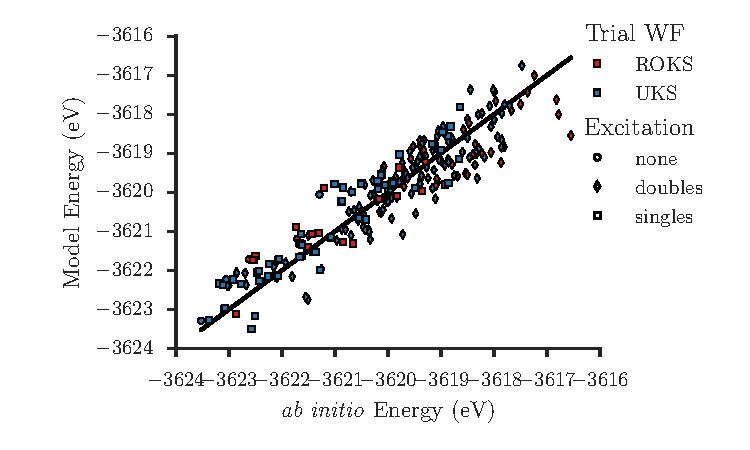
\includegraphics[width=0.7\textwidth]{./Figures/fese.pdf}
  \caption{
    Comparison of \textit{ab initio} (x-axis) and fitted energies (y-axis) of the FeSe diatomic molecule.
    \BDB{Possibly simplify this by removing UKS/ROKS}
  }
  \label{fig:fese}
\end{figure*}
